\section{Auswertung}
\label{sec:Auswertung}
Im Folgenden werden die einzelnen Messreihen ausgewertet. Dazu zählt die Kalibration des Detektors, die Bestimmung der Vollenergienachweiswahrscheinlichkeit,
die Untersuchung einer Cäsium-137 Probe und die Untersuchung von zwei unbekannten Proben.
\subsection{Kalibration des Detektors}
Um den Detektor zu kalibrieren, wird eine Europium-152 Spektrum untersucht. Hierfür wird das Spektrum in Abhängigkeit des 
Kanals geplottet und die Photonenpeaks werden herrausgesucht. Da zwischen den Kanälen des Detektor und der Energie 
der gemessenen Photonen ein linearer Zusammenhang besteht, kann eine lineare Ausgleichskurve bestimmt werden.
Das gemessene Spektrum ist in folgender Abbildung dargestellt.
\FloatBarrier
\begin{figure}
  \centering
  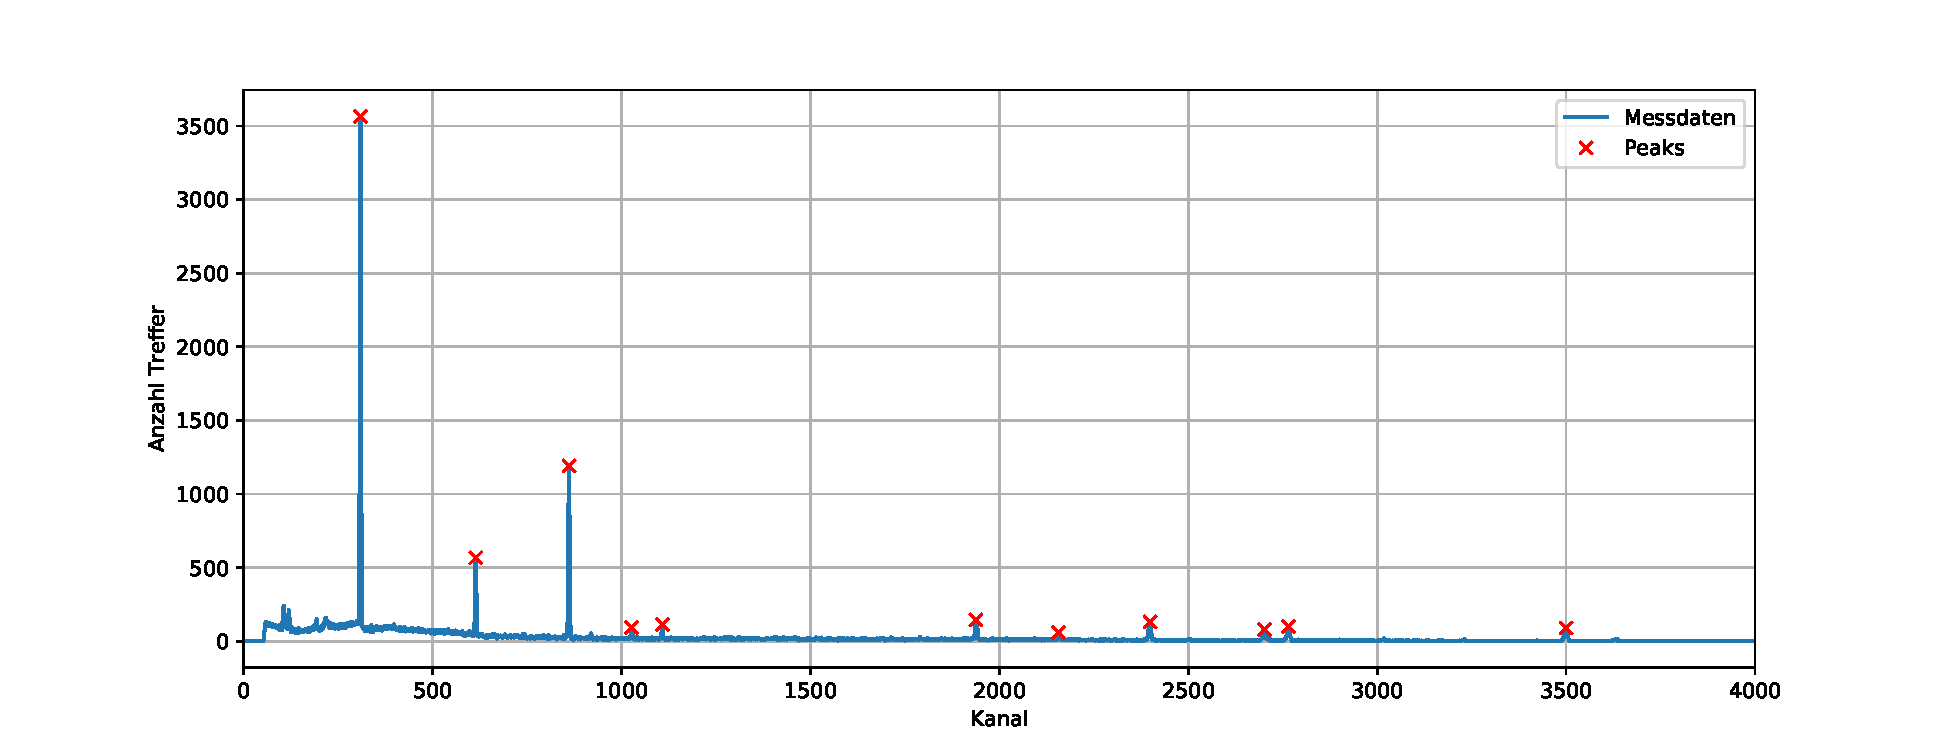
\includegraphics[width = \textwidth,keepaspectratio]{figure/Peaks_01.pdf}
  \caption{Spektrum des Europium-152 Strahlers für die Kalibration des Detektors.}
  \label{fig:Peaks_01}
\end{figure}
\FloatBarrier
Um die Peaks eindeutig zu bestimmen helfen charakteristische nahe beieinander liegende Peaks.
Die Literaturwerte der einzelnen Photonenenergien werden in Quelle \cite{Gamma_lit} dargestellt.
Die identifizierten Peaks sind in Tabelle \ref{tab:peaks_01} aufgelistet.
\FloatBarrier
\begin{table}
  \centering
  \caption{Identifizierte Peaks für die Kalibration des Detektors.}
  \label{tab:peaks_01}
  \begin{tabular}{c c c c}
    \toprule
    Peaknummer&Kanal&Energie / $\SI{}{\kilo\eV}$&Intensität / \%\\
    \midrule
    0  &309   &$\num{121.8}$&$\num{28.41}$\\
    1   &614   &$\num{244.7}$&$\num{7.55}$\\
    2   &861   &$\num{344.3}$&$\num{26.59}$\\
    3   &1027  &$\num{411.1}$&$\num{2.24}$\\
    4   &1108  &$\num{444.0}$&$\num{3.12}$\\
    5   &1938  &$\num{778.9}$&$\num{12.97}$\\
    6   &2157  &$\num{867.4}$&$\num{4.24}$\\
    7   &2399  &$\num{964.1}$&$\num{14.5}$\\
    8   &2701  &$\num{1085.8}$&$\num{10.13}$\\
    9  &2765  &$\num{1112.1}$&$\num{13.41}$\\
    10  &3500  &$\num{1408.0}$&$\num{20.9}$\\
    \bottomrule
  \end{tabular}
\end{table}
Aus Tabelle \ref{tab:peaks_01} wird die Energie gegen den Kanal geplottet und eine lineare Funktion wird an die Daten 
angepasst.
\begin{equation*}
  \label{eq:linear}
  E(k) = m\cdot k + b
\end{equation*}
\FloatBarrier
\begin{figure}
  \centering
  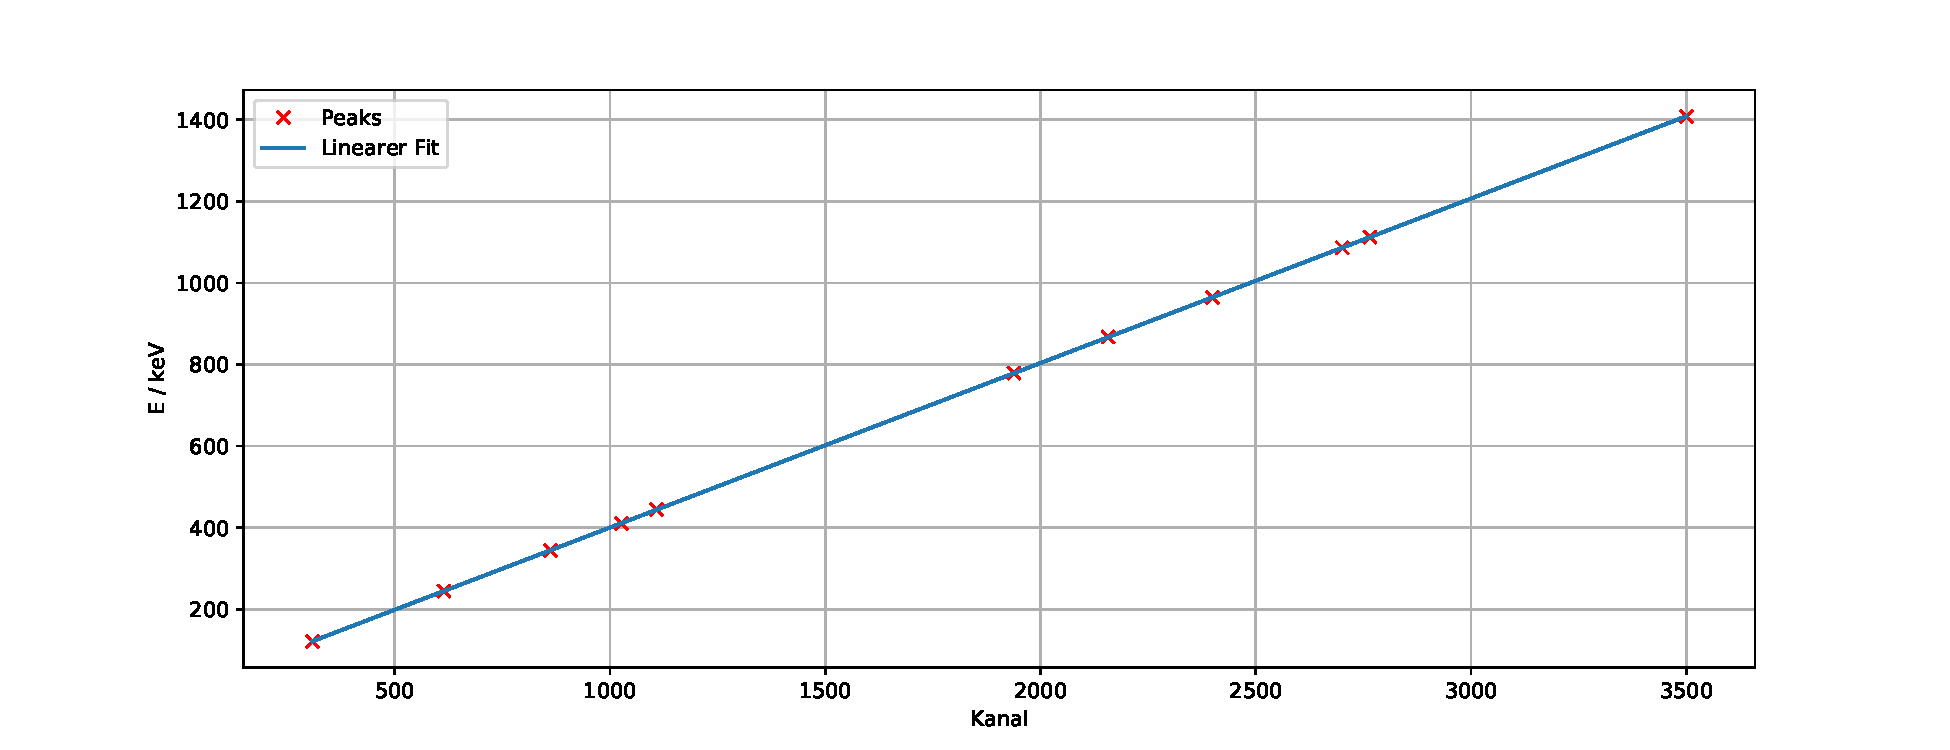
\includegraphics[width=\textwidth,keepaspectratio]{figure/Lin_Fit_01.pdf}
  \caption{Messdaten und Fitfunktion für die Kalibration des Detektors.}
  \label{fig:Lin_Fit:01}
\end{figure}
\FloatBarrier
die Fitparameter der Funktion aus \ref{fig:Lin_Fit:01} sind:
\begin{equation*}
  m = \SI{0.40312(9)}{\kilo\eV} \quad b = \SI{-2.7(1)}{\kilo\eV}
\end{equation*}
Dadurch kann das Spektrum auch gegen die Energie aufgetragen werden.
\subsection{Vollenergienachweiswahrscheinlichkeit}
\label{cap:Vollenergienachweiswahrscheinlichkeit}
Die Europium-152 Probe hatte am 01.10.2000 eine Aktivität von $\SI{4130(60)}{\becquerel}$. Mit einer 
Halbwertszeit von $T_{1/2} = \SI{13.52}{yr}$ kann über das Zerfallsgesetzt die Aktivität 
am Messtag bestimmt werden, diese liegt bei $\SI{1552(20)}{\becquerel}$.
Um die Vollenergienachweiswahrscheinlichkeit $\eta(E)$ bestimmen zu können, wird folgende Formel benötigt.
\begin{equation}
  \label{eq:eta_N}
  N = tA_{\text{Messtag}}I\frac{\Omega}{4\pi}\eta(E)
\end{equation}
Hierbei ist $t=\SI{4109.4111}{\second}$ die Messzeit, $I$ die Intensität  des Peaks und $\Omega$ der vom Detektor abgedeckter
Raumwinkel.
Da die Probe als punktförmig angesehen werden kann, kann $\Omega$ mithilfe der Formel \eqref{eq:Omega} bestimmt werden.
\begin{equation}
  \label{eq:Omega}
  \Omega = \int_{0}^{2\pi}\int_{0}^{\frac{\theta}{2}} \sin\left(\theta'\right)\symup{d}\theta'\symup{d}\varphi = 
  2\pi \left(1-\cos\left(\frac{\theta}{2}\right)\right)
\end{equation}
Mit der Winkelbeziehung 
\begin{equation*}
  \tan\left(\frac{\theta}{2}\right) = \frac{r}{d} \implies \frac{\theta}{2} = \arctan\left(\frac{r}{d}\right)
\end{equation*}
und den Werten $d = \SI{8}{\centi\meter}$ und $r = \SI{2.25}{\centi\meter}$ kann $\Omega$ bestimmt werden.
\begin{equation*}
  \Omega = 2\pi \left(1-\cos\left(\frac{\theta}{2}\right)\right) = 2\pi\left(1- \frac{1}{\sqrt{\left(\frac{r}{d}\right)^2+1}}\right) \approx \num{0.23}
\end{equation*}
Um den Linieninhalt $N$ zu bestimmen wird eine Gaußglocke \eqref{eq:Gauß} an die Daten angepasst.
\begin{equation}
  \label{eq:Gauß}
  n(k)= A_0 \symup{e}^{-c(k-k_0)^2} + b
\end{equation}
Die Fits sind in Abbildung \ref{fig:subplots_01} zu sehen.
\FloatBarrier
\begin{figure}
  \centering
  \caption{Ausgleichskurven für die Bestimmung des Linieninhaltes $N$.}
  \label{fig:subplots_01}
  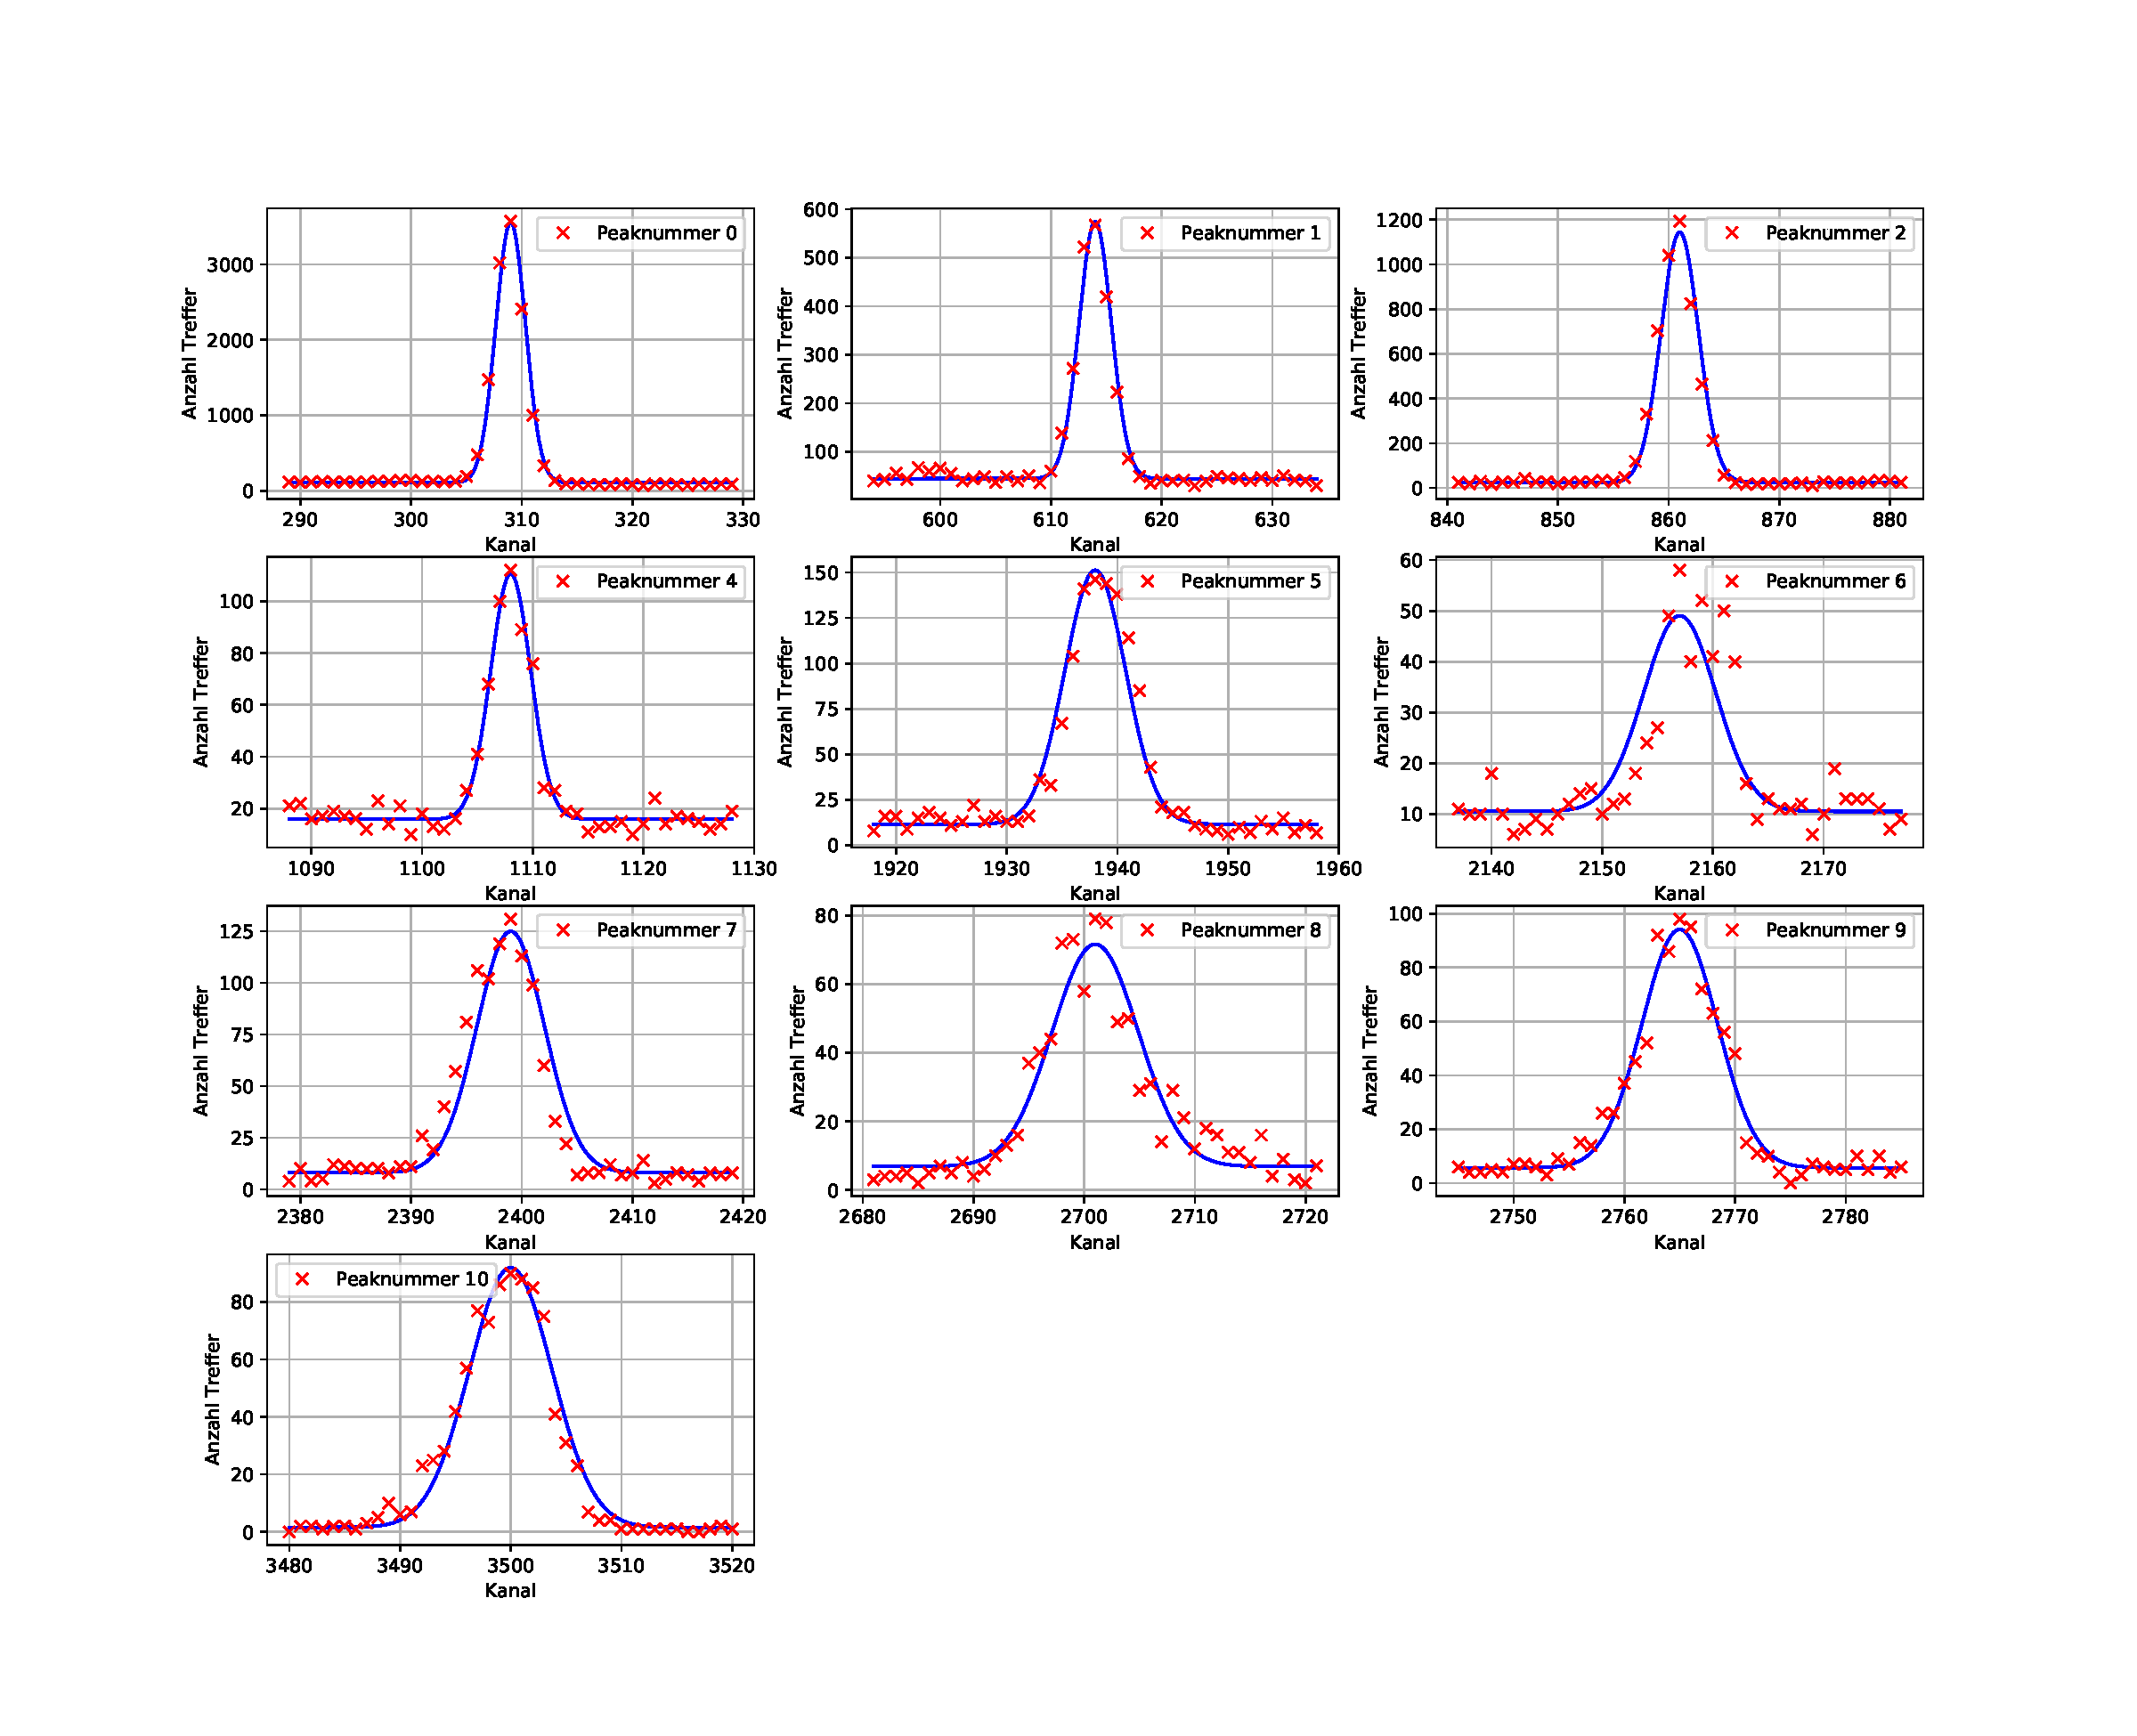
\includegraphics[width=\textwidth,keepaspectratio]{figure/Subplot_01.pdf}
\end{figure}
\FloatBarrier
Die Fitparameter sind in Tabelle \ref{tab:fit_params} aufgelistet. Mit der Gleichung 
\begin{equation*}
  N = A_0\sqrt{\frac{\pi}{c}}
\end{equation*}
kann der Linieninhalt bestimmt werden. Bei Peaknummer 3 ist der Fitparameter $c$ negativ und wird daher verworfen.
\FloatBarrier
\begin{table}
  \centering
  \caption{Fitparameter und Linieninhalte der einzelnen Peaks.}
  \label{tab:fit_params}
  \begin{tabular}{c c c c c}
    \toprule
    Peaknummer&$A_0$&$c$&$b$&$N$\\
    \midrule
    0   &$\num{3.45(7)e+03} $&$\num{0.277(14)}$ &$\num{105(10)}$&$\num{1.16(4)e+04}$\\
    1   &$\num{530(10)}     $&$\num{0.235(13)}$ &$\num{45(3)}$&$\num{1.94(7)e+03}$\\  
    2   &$\num{1121(30)}    $&$\num{0.175(11)}$ &$\num{24(7)}$&$\num{4.75(20)e+03}$\\
    4   &$\num{95.0(3)}     $&$\num{0.153(12)}$ &$\num{16(1)}$&$\num{430(20)}$\\
    5   &$\num{140(6)}      $&$\num{0.066(6)}$  &$\num{12(2)}$&$\num{9.7(6)e+02}$\\
    6   &$\num{39(4)}       $&$\num{0.047(11)}$ &$\num{11(1)}$&$\num{3.2(5)e+02}$\\
    7   &$\num{117(6)}      $&$\num{0.054(6)}$  &$\num{8(2)}$&$\num{8.9(7)e+02}$\\
    8   &$\num{65(4)}       $&$\num{0.033(5)}$  &$\num{7(2)}$&$\num{6.3(6)e+02}$\\
    9   &$\num{88(3)}       $&$\num{0.0430(30)}$&$\num{6(1)}$&$\num{7.5(4)e+02}$\\
    10  &$\num{90(2)}       $&$\num{0.0360(20)}$&$\num{2(1)}$&$\num{841(30)}$\\
    \bottomrule
  \end{tabular}
\end{table}
\FloatBarrier
Mit der Gleichung \eqref{eq:eta_N} können $\eta$-Werte bestimmt werden, an diese wird die Funktion 
\begin{equation*}
  \eta(E) = A\cdot E ^z
\end{equation*}
angepasst. 
Die Fitparameter für den Fit aus Abbildung \ref{fig:Vollenergienachweiswahrscheinlichkeit} sind 
\begin{equation*}
  A = \num{0.22(4)} \quad z = \num{-0.86(3)}.
\end{equation*}
\begin{figure}
  \centering
  \caption{Messwerte und Fitfunktion für die Bestimmung der Vollenergienachweiswahrscheinlichkeit.}
  \label{fig:Vollenergienachweiswahrscheinlichkeit}
  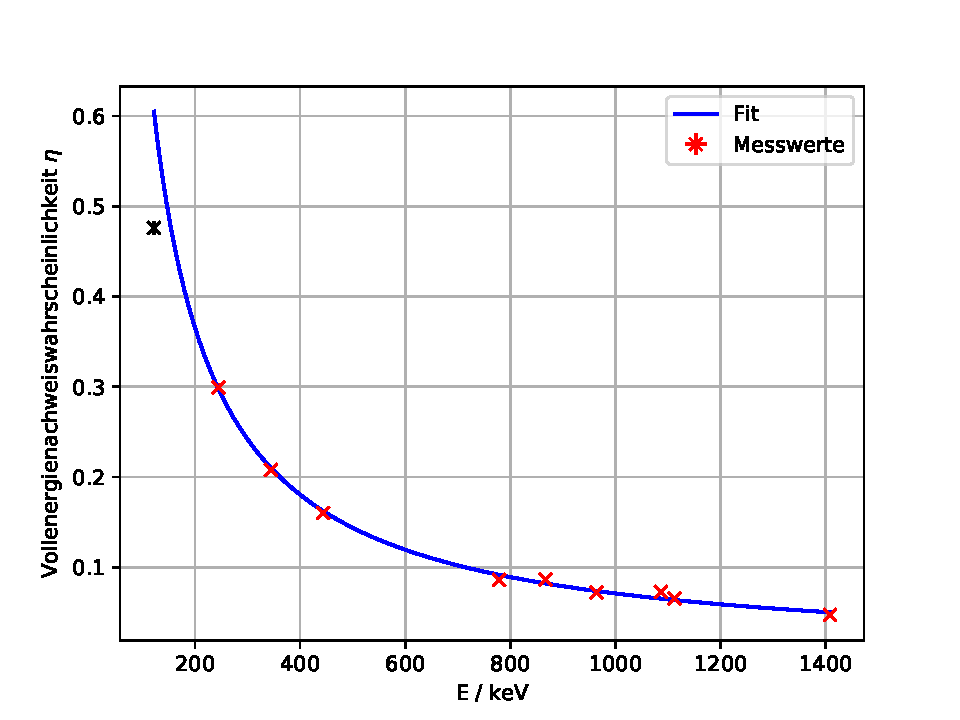
\includegraphics[width = \textwidth, keepaspectratio]{figure/Vollenergienachweiswahrscheinlichkeit.pdf}
\end{figure}
\FloatBarrier
\subsection{Untersuchung der Cäsium-137 Probe}
Das gemessene Spektrum ist in Abbildung \ref{fig:Cs137} dargestellt.
\FloatBarrier
\begin{figure}
  \centering
  \caption{Spektrum der Cäsium-137 Probe, hierbei wird der Kanal direkt in eine Energie umgerechnet.}
  \label{fig:Cs137}
  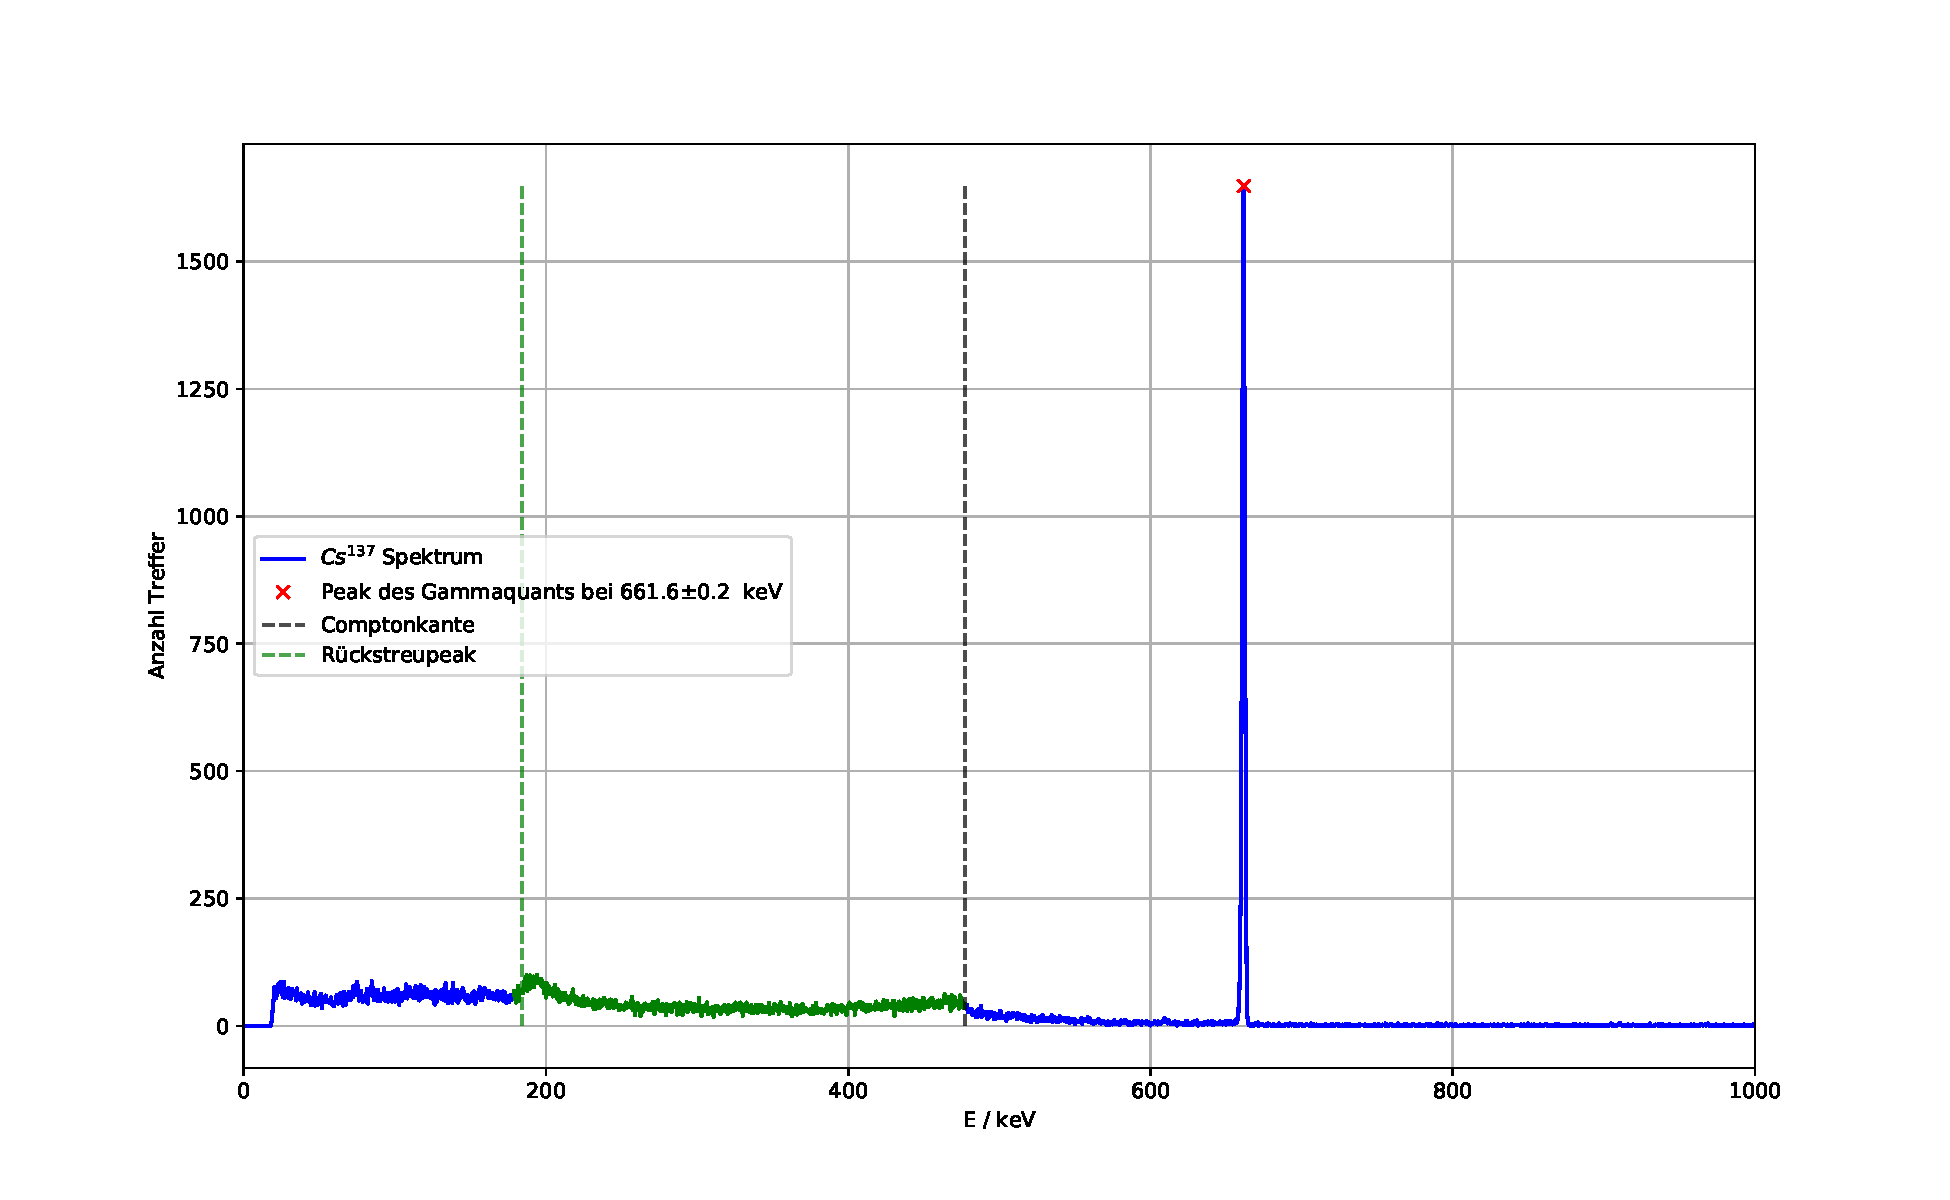
\includegraphics[width= \textwidth,keepaspectratio]{figure/02_peaks.pdf}
\end{figure}
\FloatBarrier
Der Photonpeak liegt bei $E_{\gamma}\SI{661.6(2)}{\kilo\eV}$. Mit den Gleichungen \eqref{3.1} und \eqref{2.9} kann 
die Comptonkante und die Rückstreuenergie bestimmt werden.
\begin{equation*}
  T_{\text{max}} = \SI{477.3(2)}{\kilo\eV} \quad E_{\text{rückstreu}} = \SI{184.32(1)}{\kilo\eV}
\end{equation*}
Wie an Abbildung \ref{fig:Cs137} zu sehen ist, stimmen die gemessenen und die berechneten Werte überein.
Für die Bestimmung der Halbwertsbreite und der Zehntelwertsbreite, wird um den Photonenpeak eine Gaußglocke der Form 
\eqref{eq:Gauß} gefittet.
Die Fitparameter aus der Abbildung \ref{fig:02_fit} sind 
\begin{equation*}
  A_0 = \num{1618(30)}\quad c = \num{0.58(2)} \quad b = \num{8(9)}
\end{equation*}
\FloatBarrier
\begin{figure}
  \centering
  \caption{Messdaten um den Photonenpeak und Gaußglockenfit für die Bestimmung der Halb-, Zehntelwertsbreite und den Linieninhalt des Peaks.}
  \label{fig:02_fit}
  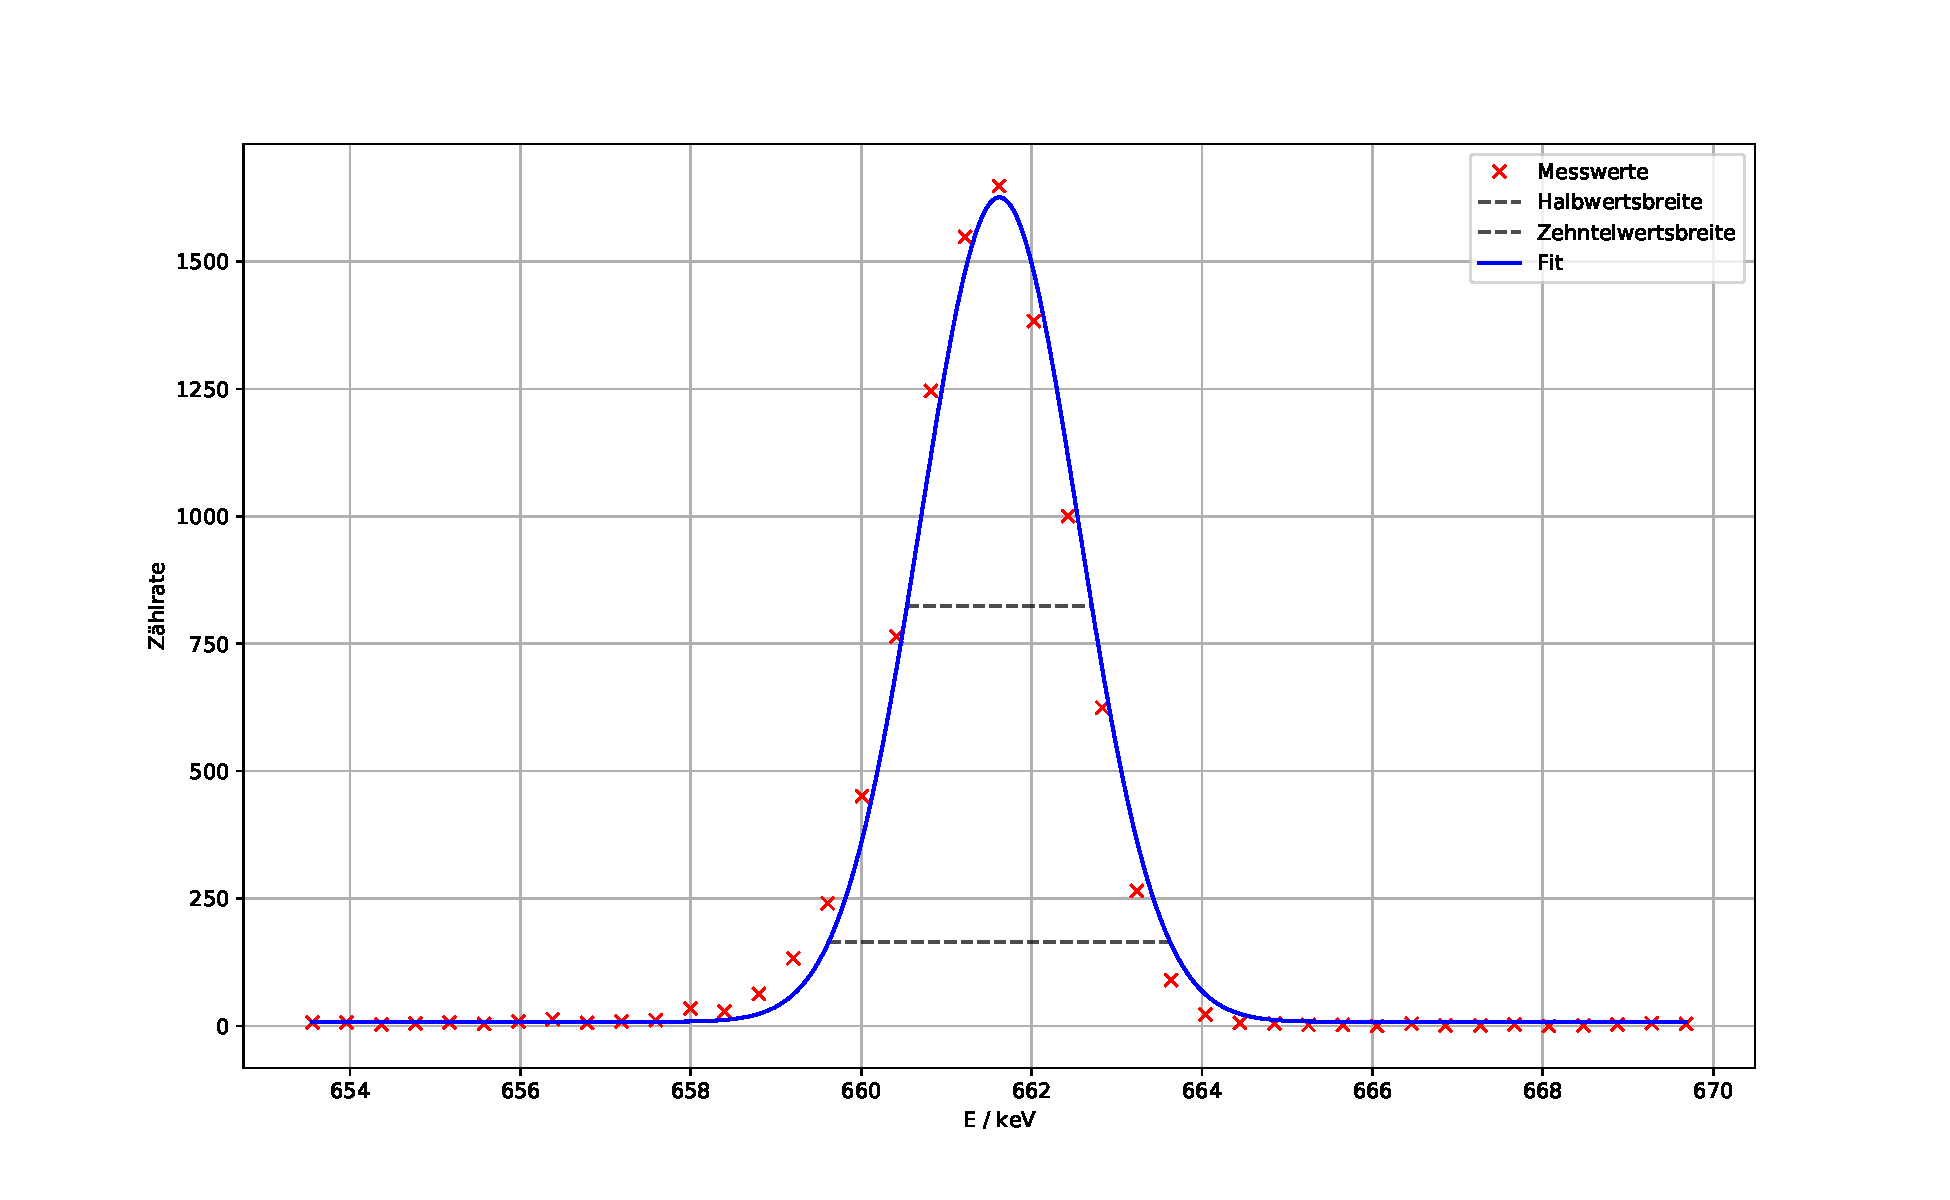
\includegraphics[width=\textwidth,keepaspectratio]{figure/02_peak_fit.pdf}
\end{figure}
\FloatBarrier
Die beiden Breiten werden bestimmt, indem die Kurve um die Hälfte, ein Zehntel des Maximalen Wertes verringert wird und auf Nullstellen 
untersucht wird.
Die Differenzen der beiden Nullstellen sind die Breiten.
\begin{equation*}
  \Gamma_{1/2} = \SI{2.17(6)}{\kilo\eV}\quad \Gamma_{1/10} = \SI{4.0(1)}{\kilo\eV}
\end{equation*}
Das Verhältnis der beiden Breiten ist $\num{1.85(2)}$, das Verhältnis der beiden Breiten bei einer Gaußglocke wird 
mit der Formel
\begin{equation*}
  \frac{\Gamma_{1/10}}{\Gamma_{1/2}}= \sqrt{\frac{\ln{10}}{\ln{2}}} \approx \num{1.82}
\end{equation*}
bestimmt.
Mit der Fitkurve aus Abbildung \ref{fig:02_fit} kann der Linieninhalt bestimmt werden. Hierbei ist darauf zu achten, dass der Fit ein zweites mal gemacht wird 
und hierbei nicht die Energie sondern der Kanal verwendet wird. Damit lässt sich der Lineninhalt des Peaks auf $N=\num{9.3(2)e3}$ bestimmen.
Um den Inhalt des Comptonkontinuums zu bestimmen wird eine Ausgleichskurve der Gleichung \eqref{ludwig/mirjam 2.12} berechnet.
Hierbei wird nur der Ausdruck vor der Klammer an den grün markierten Bereich aus \ref{fig:Cs137} angepasst.
Der bestimmte Parameter lautet $B=\num{1617.8(3)}$. Um den Inhalt der Funktion \ref{ludwig/mirjam 2.12} zu erhalten,
werden alle Werte bis zur Comptonkante aufaddiert. Der Inhalt ist damit $N_{\text{Comp}} = \num{2.2495(5)e6}$.
Mit der Photonenenergien $E_{\gamma}\SI{661.6(2)}{\kilo\eV}$ und der Hilfe der Gleichungen \eqref{ludwig/mirjam 2.4} und 
\eqref{ludwig/mirjam 2.10} kann der Wirkungsquerschnitt des Compoton-Effekts und des Photoeffekts bestimmt werden.
Diese liegen bei 
\begin{equation*}
  \sigma_{\text{Comp}}=\SI{8.196(1)}{b} \quad \sigma_{\text{Photo}}=\SI{0.05674(6)}{b}.
\end{equation*} 
Mit der Annahme das die Dichte von Germanium im Detektor bei $\rho = \SI{5.323}{\gram\per\cubic\centi\meter}$ [Quelle suchen] liegt und der
Gleichung \eqref{ludwig/mirjam 2.3} kann der Extinktionskoeffizient bestimmt werden.
Diese liegen bei 
\begin{equation*}
  \mu_{\text{Comp}} = \SI{0.35514(6)}{cm^{-1}} \quad \mu_{\text{Photo}} = \SI{0.002459(2)}{cm^{-1}}.
\end{equation*}
Mit diesen Werten und der Gleichung \eqref{ludwig/mirjam 2.2} kann die Wechselwirkungswahrscheinlichkeit bestimmt werden.
Hierbei ist $l=\SI{3.9}{\centi\meter}$ die Länge des Germanium-Kristalls.
Die Wechselwirkungswahrscheinlichkeiten sind 
\begin{equation*}
  P_{\text{Comp}} = \num{0.74968(5)}\quad P_{\text{Photo}} = \num{0.00954(1)}.
\end{equation*}
Das Verhältnis der beiden Größen ist
\begin{equation*}
  \frac{P_{\text{Comp}} }{P_{\text{Photo}}} = \num{78.56(8)}.
\end{equation*}
\subsection{Aktivitätsbestimmung}
Bei diesem Versuchsteil wird zunächst, anhand der Gamma-Linien, das untersuchte Material bestimmt.
Möglich sind Antimon-125 oder Barium-133.
Die verwendeten Gamma Peaks der beiden potentiellen Proben sind in Tabelle \ref{tab:Ba_133Sb_125} aufgelistet.
\FloatBarrier
\begin{table}
  \centering
  \caption{Energie und Intensität der beiden potenteillen Proben.}
  \label{tab:Ba_133Sb_125}
  \begin{tabular}{c c c c c}
    \toprule
    & \multicolumn{2}{c}{Antimon-125} & \multicolumn{2}{c}{Barium-133} \\
    \cmidrule(lr){2-3}\cmidrule(lr){4-5}
    Peaknummer & E / \SI{}{\kilo\eV} & Intensität / \%& E / \SI{}{\kilo\eV} & Intensität / \%\\
    \midrule
    0&$\num{427.874}$&$\num{29.55}$&$\num{356.0129}$&$\num{62.05}$\\
    1&$\num{600.597}$&$\num{17.76}$&$\num{80.9979}$&$\num{33.31}$\\
    2&$\num{635.950}$&$\num{11.32}$&$\num{302.8508}$&$\num{18.31}$\\
    3&$\num{463.365}$&$\num{10.48}$&$\num{383.8485}$&$\num{8.94}$\\
    4&$\num{176.314}$&$\num{6.82}$ &$\num{276.3989}$&$\num{7.13}$\\
    5&$\num{35.489}$&$\num{5.79}$  &\textcolor{orange}{$\num{79.6142}$}&\textcolor{orange}{$\num{2.63}$}\\
    6&$\num{606.713}$&$\num{5.02}$ &\textcolor{orange}{$\num{53.1622}$}&\textcolor{orange}{$\num{2.14}$}\\
    7&$\num{671.441}$&$\num{1.783}$&$\num{160.6121}$&$\num{0.638}$\\
    8&$\num{380.452}$&$\num{1.520}$&\textcolor{orange}{$\num{223.2368}$}&\textcolor{orange}{$\num{0.450}$}\\
    \bottomrule
  \end{tabular}
\end{table}
\FloatBarrier
Um die Probe zu identifizieren werden die Peaks im gemessenen Spektrum markiert, dies ist in Abbildung \ref{fig:03_peaks} zu sehen.
\FloatBarrier
\begin{figure}
  \centering
  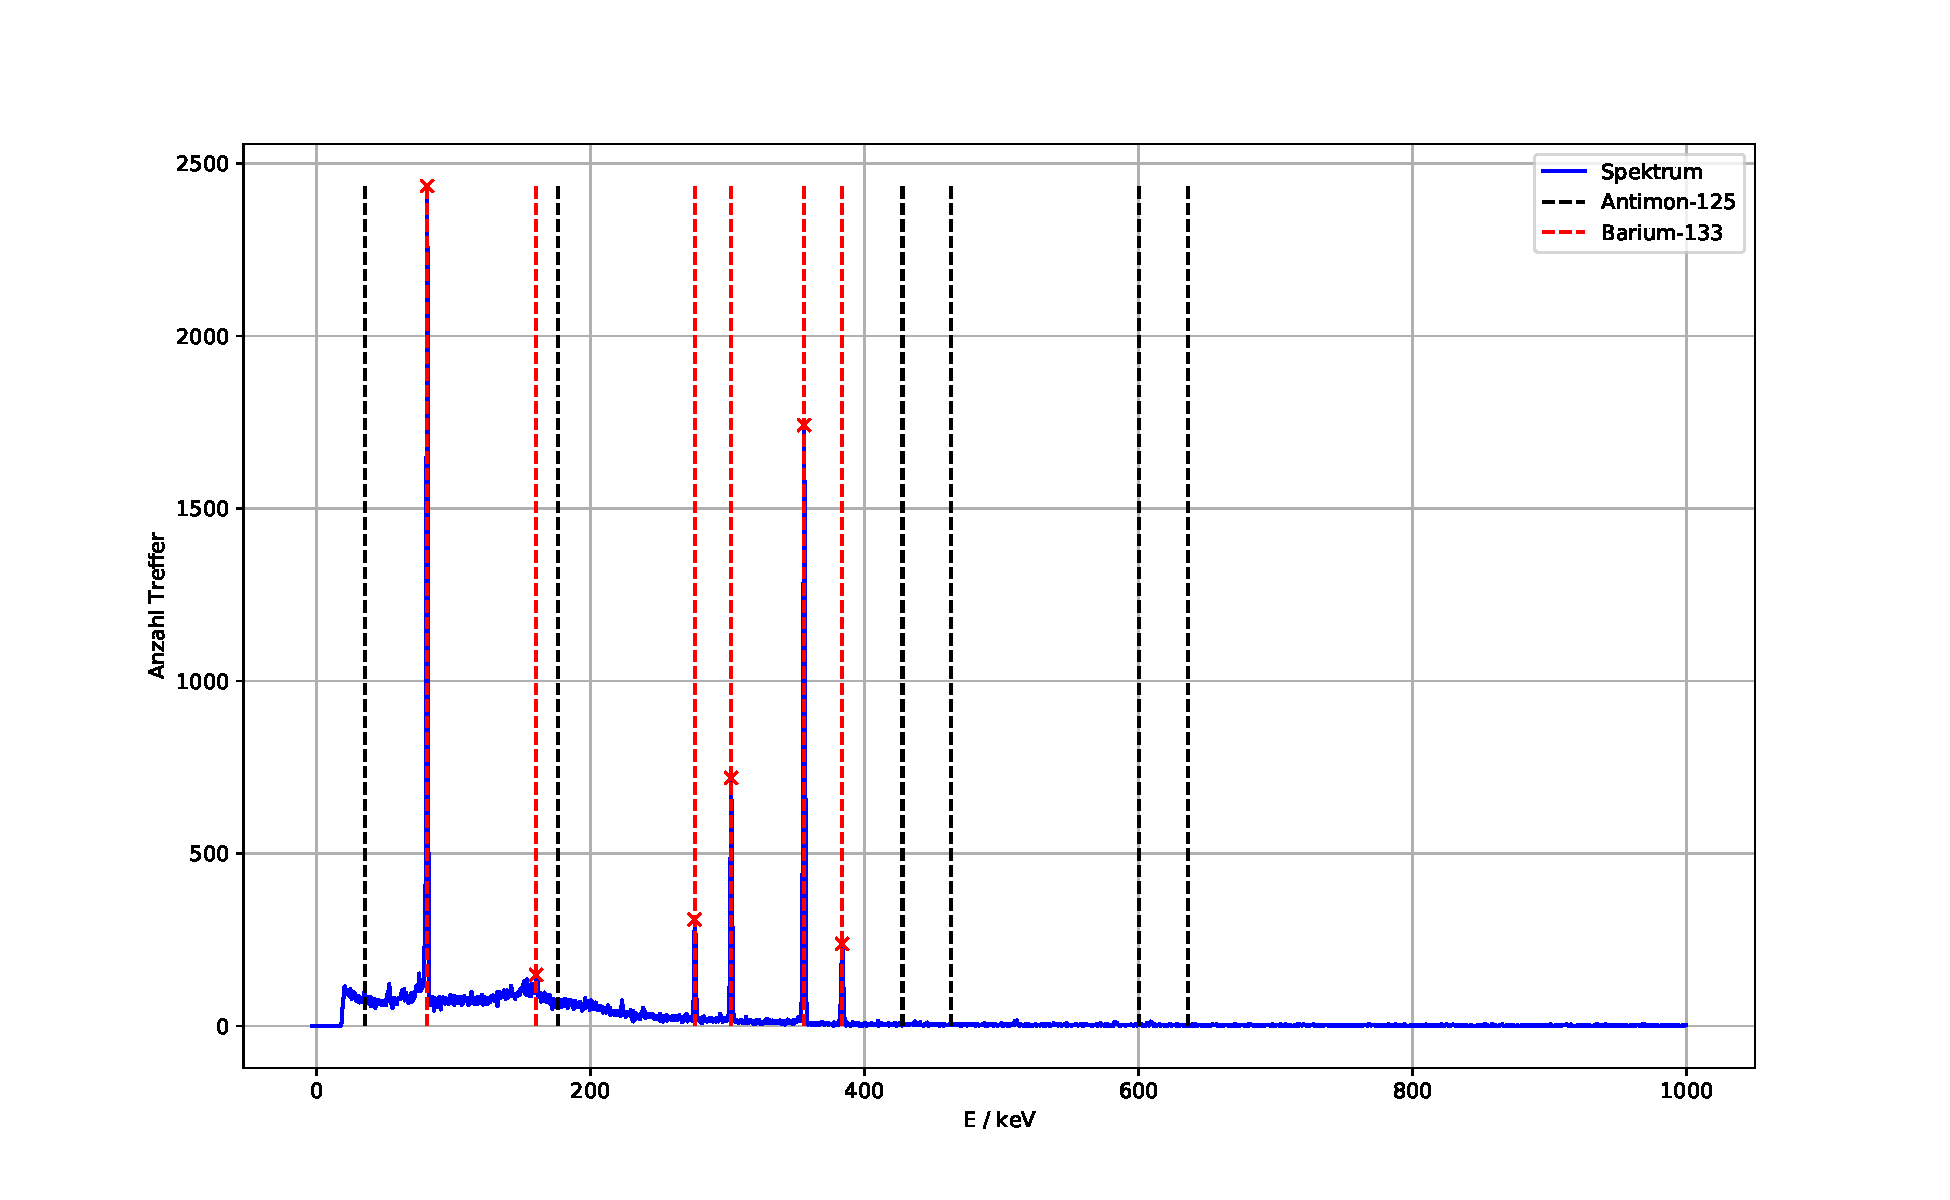
\includegraphics[width = \textwidth, keepaspectratio]{figure/03_peaks.pdf}
  \caption{Aufgenommenes Spektrum mit den Literaturwerten der Gamma-Peaks, hierbei konnten alle Peaks von Barium-133 (außer die orange markierten) aus Tabelle \ref{tab:Ba_133Sb_125} identifiziert werden.}
\end{figure}
\FloatBarrier
Um die Aktivität zu bestimmen, wird die Gleichung \eqref{eq:eta_N} verwendet. Hierbei ist die Messzeit $t=\SI{3770.3771}{\second}$, 
$\Omega$ ist wie in vorherigen Teilen bestimmt worden und die Intensitäten werden aus Tabelle \ref{tab:Ba_133Sb_125} abgelesen.
Die Funktion für die Vollenergienachweiswahrscheinlichkeit wurde bereits in Kapitel \ref{cap:Vollenergienachweiswahrscheinlichkeit}
bestimmt.
Der Linieninhalt wird bestimmt wie in den vorherigen Kapitel.
Die Fits für die Bestimmung der Linieninhalt, sowie die Linieninhalte selbst, sind in Tabelle \ref{tab:params_Linieninhalt} aufgelistet.
\FloatBarrier
\begin{table}
  \centering
  \caption{Fitparameter für die Bestimmung der Linieninhalte.}
  \label{tab:params_Linieninhalt}
  \begin{tabular}{c c c c c}
    \toprule
    Peaknummer&$A_0$&$c$&$b$&$N$\\
    \midrule
    0&$\num{2.32(10)e+03}$&$\num{0.311(31)}$   &$\num{102(20)}$&$\num{2.34(26)e+04}$\\
    1&$\num{0(3)e+08}$   &$\num{-0.0000(29)}$&$\num{0(3)e+08}$&$---$\\
    2&$\num{286(15)}$     &$\num{0.226(27)}$  &$\num{21(3)}$&$\num{4.0(5)e+03}$\\
    3&$\num{682(10)}$     &$\num{0.218(8)}$   &$\num{17(2)}$&$\num{9.8(4)e+03}$\\
    4&$\num{1769(9)}$     &$\num{0.1834(22)}$ &$\num{9.7(21)}$&$\num{3.03(4)e+04}$\\
    7&$\num{230(5)}$      &$\num{0.186(9)}$   &$\num{6.3(12)}$&$\num{3.90(21)e+03}$\\
    \bottomrule
  \end{tabular}
\end{table}
\FloatBarrier
Die Fits für die Bestimmung der Lineninhalte sind in Abbildung \ref{fig:Linieninhalt_03} dargestellt.
\FloatBarrier
\begin{figure}
  \centering
  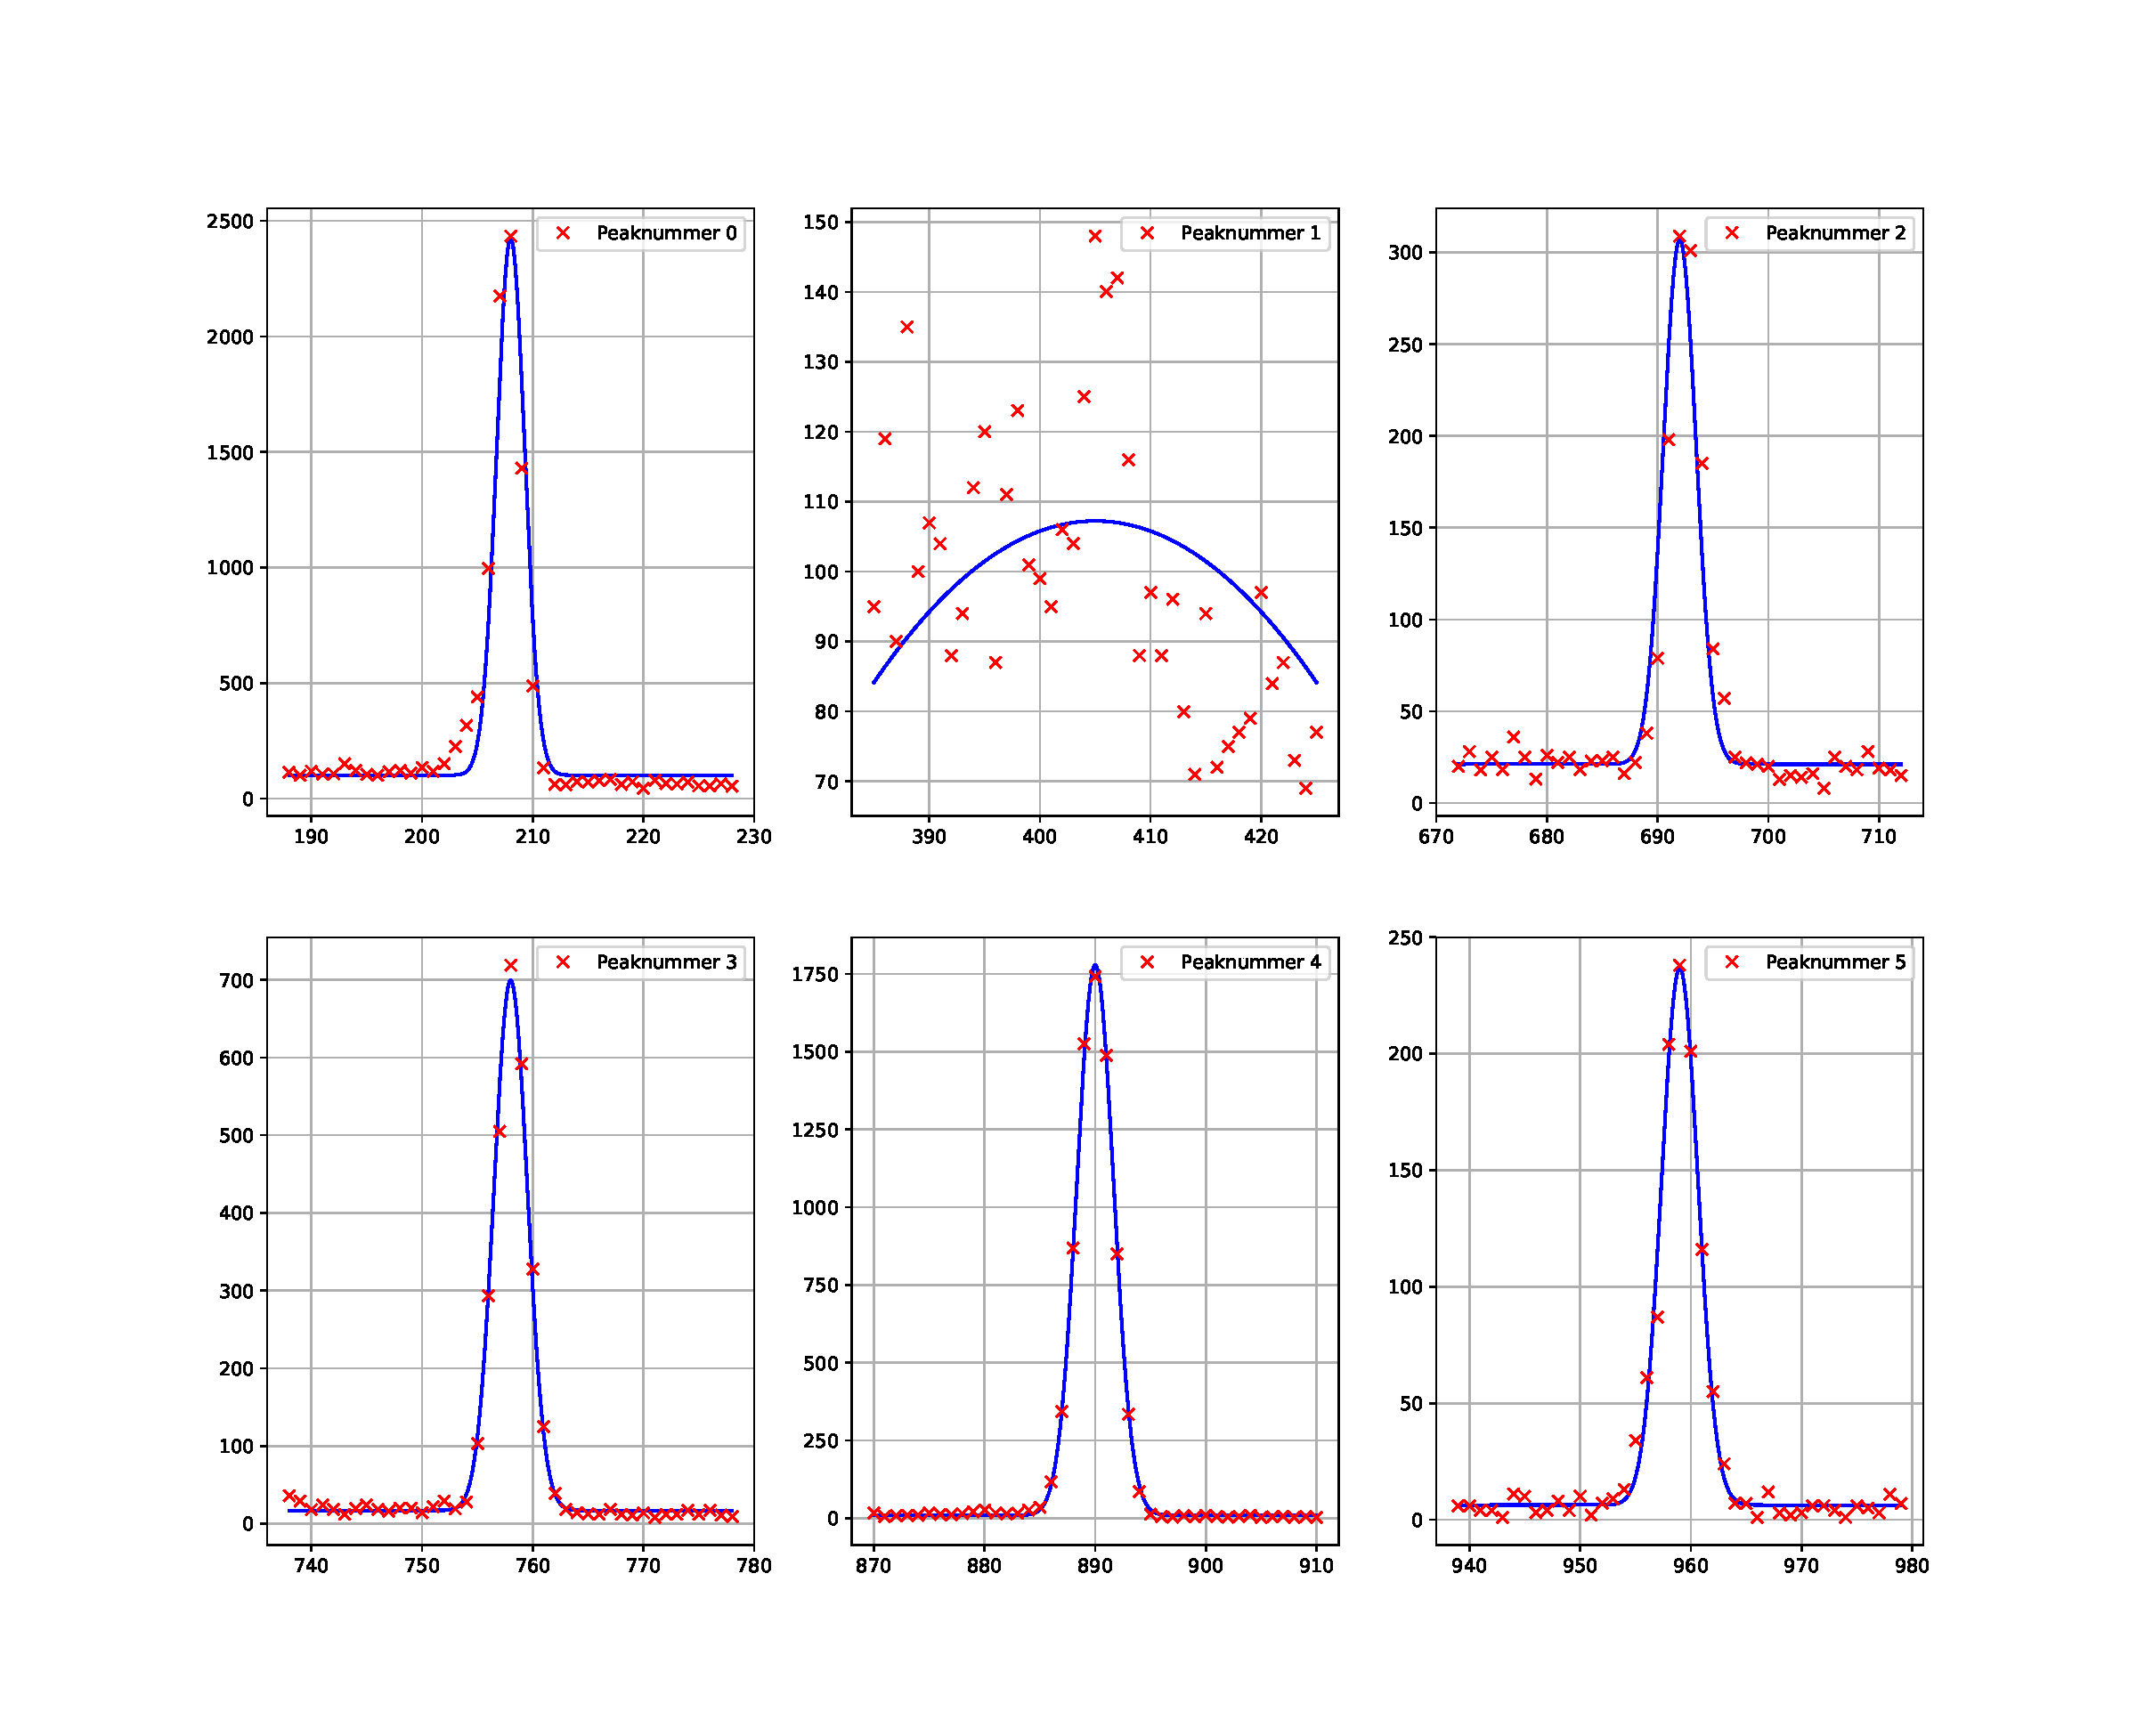
\includegraphics[width=\textwidth,keepaspectratio]{figure/03_subplot.pdf}
  \caption{Fits für die Bestimmung der Lineninhalte.}
  \label{fig:Linieninhalt_03}
\end{figure}
Mit den berechneten Linieninhalten kann mit der Gleichung \eqref{eq:eta_N} die Aktivität am Messtag bestimmt werden. 
Diese sind in Tabelle \ref{tab:Akti_03} aufgelistet.
\FloatBarrier
\begin{table}
  \centering
  \caption{Aktivität der Barium-133 Probe. Bestimmt über die einzelnen Peaks und gemittelt.}
  \label{tab:Akti_03}
  \begin{tabular}{c c}
    \toprule
    Peaknummer & Aktivität / $\SI{}{\becquerel}$\\
    \midrule
    0&$\num{6.3(15)e+02}$\\
    2&$\num{1.22(32)e+03}$\\
    3&$\num{1.25(33)e+03}$\\
    4&$\num{1.20(32)e+03}$\\
    7&$\num{1.15(31)e+03}$\\
    \midrule
    mittel& $\num{1.09(28)e+03}$\\
    \bottomrule
  \end{tabular}
\end{table}
\subsection{Bestimmung einer unbekannten Probe}
Bei diesem Versuchsteil wird nur  das Material der Probe bestimmt, da aufgrund der Ausdehnung der Probe diese nicht als Punktförmig 
angesehen werden kann und damit $\Omega$ nicht berechnet werden kann, was eine notwendige Größe für die Bestimmung der Aktivität ist.
Das Spektrum ist in Abbildung \ref{fig:Peaks_04} zu sehen.
Von den gefundenen Peaks können neun Peaks identifiziert werden. Diese sind in Tabelle \ref{tab:ident_Peaks} 
aufgelistet.
\FloatBarrier
\begin{table}
  \centering
  \caption{Energien der identifizierten Peaks aus dem Spektrum und die dazugehörigen Literaturwerte \cite{}[Nuklid Karte].}
  \label{tab:ident_Peaks}
  \begin{tabular}{c c c c}
    \midrule
    Isotop& Energie (gemessen) / $\SI{}{\kilo\eV}$&  Energie (Lit.) / $\SI{}{\kilo\eV}$& Intensität (Lit.) / \%\\
    \midrule
    234Th&$\num{92.8(1)}$&$\num{92.8}$&$\num{3.75}$\\
    (235U)&$\num{185.94(18)}$&$\num{185.72}$&$\num{57.0}$\\
    226Ra&$\num{185.94(18)}$&$\num{186.21}$&$\num{3.6}$\\
    214Pb&$\num{241.97(19)}$&$\num{242.00}$&$\num{7.3}$\\
    214Pb&$\num{295.19(19)}$&$\num{295.22}$&$\num{18.4}$\\
    214Pb&$\num{352.03(20)}$&$\num{351.93}$&$\num{35.6}$\\
    214Bi&$\num{609.22(23)}$&$\num{609.31}$&$\num{45.5}$\\
    (214Rn)&$\num{609.22(23)}$&$\num{609.31}$&$\num{0.1}$\\
    214Bi&$\num{665.65(25)}$&$\num{665.45}$&$\num{1.5}$\\
    214Bi&$\num{768.05(25)}$&$\num{768.36}$&$\num{4.9}$\\
    214Pb&$\num{786.19(25)}$&$\num{785.96}$&$\num{1.1}$\\
    234Pa&$\num{805.5(2)}$&$\num{805.8}$&$\num{2.5}$\\
    214Bi&$\num{806.34(26)}$&$\num{806.17}$&$\num{1.3}$\\
    214Bi&$\num{934.94(28)}$&$\num{934.06}$&$\num{3.1}$\\
    214Bi&$\num{1120.78(31)}$&$\num{1120.29}$&$\num{14.9}$\\
    214Bi&$\num{1238.89(33)}$&$\num{1238.11}$&$\num{5.8}$\\
    214Bi&$\num{1377.6(4)}$&$\num{1377.7}$&$\num{4.0}$\\
    214Bi&$\num{1764.6(4)}$&$\num{1764.49}$&$\num{15.31}$\\
    \bottomrule
  \end{tabular}
\end{table}
\begin{figure}
  \centering
  \caption{gemessenes Spektrum einer unbekannten Probe.}
  \label{fig:Peaks_04}
  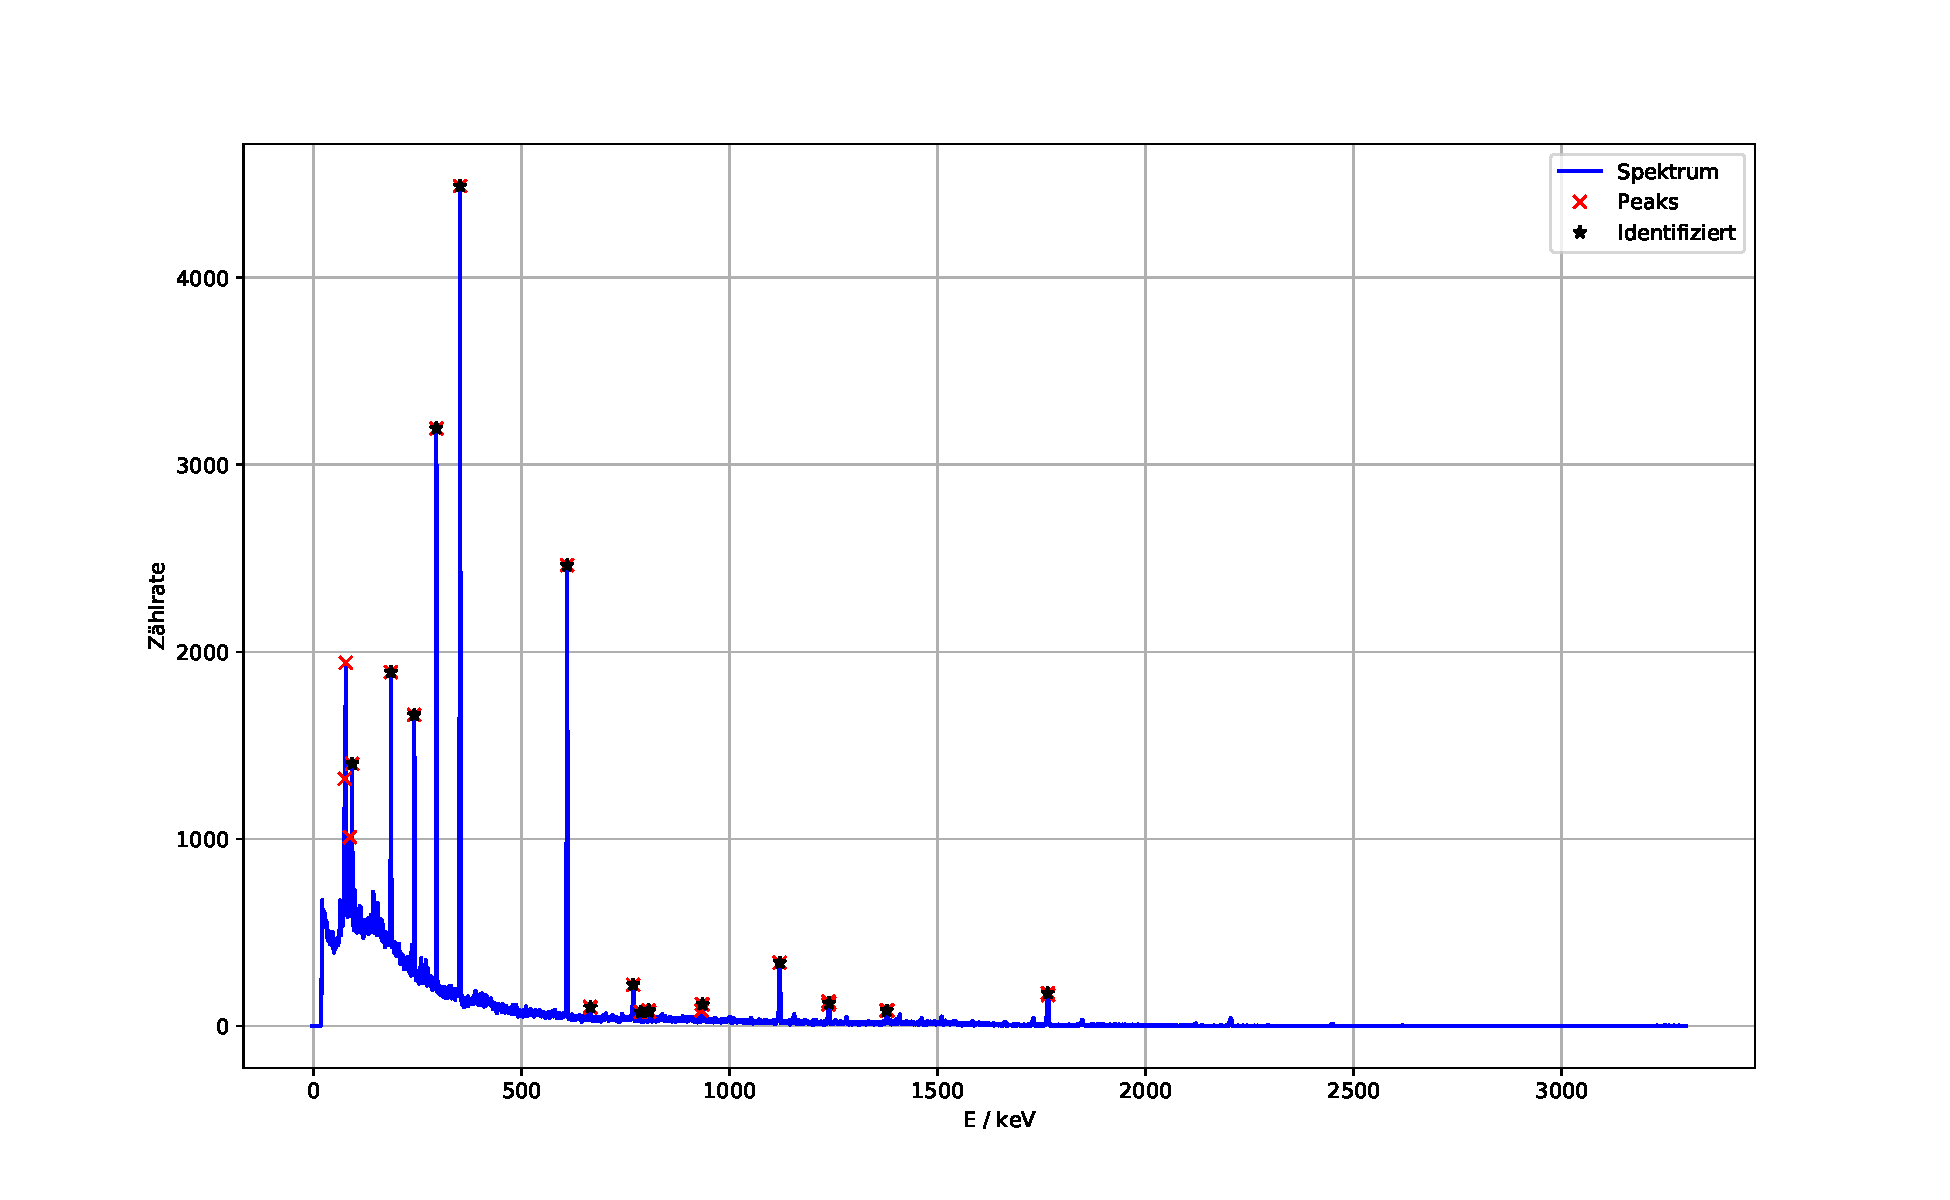
\includegraphics[width=\textwidth,keepaspectratio]{figure/04_peaks.pdf}
\end{figure}
\FloatBarrier
Die Isotope aus Tabelle \ref{tab:ident_Peaks} gehören alle zu der natürlichen Zerfallsreihe des Uran Isotop Uran-238, 
außer der Peak von Uran-235 bei einer Energie von $\SI{185.94(18)}{\kilo\eV}$. Dieser Peak kann allerdings einem anderen 
Isotop zugeordnet werden Radium-226, welches zu der Zerfalls von Uran-238 gehört.








